\documentclass[journal]{IEEEtran}
\usepackage{cite}
\usepackage{amssymb}
\usepackage{amsmath}
\usepackage{graphicx}

\graphicspath{ {figures/} }

\title{Optimizing Compressed Sensing Projection Matrices}
\author{Nicholas McKibben and Connor Anderson}

\begin{document}
\maketitle
\thispagestyle{empty}
\pagestyle{empty}
%%%%%%%%%%%%%%%%%%%%%%%%%%%%%%%%%%%%%%%%%%%%%%%%%%%%%%%%%%%%%%%%%%%%%%%%%%%%%%%%
\begin{abstract}

Compressed Sensing (CS) is a technique for reconstructing a signal that has been sampled well below the Nyquist-Shannon criterion.  In general, it is impossible to recover an undersampled signal.  However, when the original signal meets certain constraints, it becomes possible to recover it from its undersampled representation with a high (or even perfect) degree of accuracy.  Compressed sensing is a method for recovering signals that have been highly undersampled and have a sparse representation in some transform domain.  Luckily, many signals of interest can be shown to have sparse representations using common transforms such as the Wavelet Transform or the Discrete Cosine Transform. If those signals are sampled in the right way, they can be represented by far fewer data points but recovered almost exactly.  This project demonstrates an algorithm that optimizes the sensing matrix for basis pursuit CS reconstruction.

\end{abstract}
%%%%%%%%%%%%%%%%%%%%%%%%%%%%%%%%%%%%%%%%%%%%%%%%%%%%%%%%%%%%%%%%%%%%%%%%%%%%%%%%

%%%%%%%%%%%%%%%%%%%%%%%%%%%%%%%%%%%%%%%%%%%%%%%%%%%%%%%%%%%%%%%%%%%%%%%%%%%%%%%%
\section{INTRODUCTION}

The notion of sparse representation and reconstruction is actually a well-studied problem within statistics, first described by Santosa and Symes in 1986 \cite{santosa}.  But the ramifications of the robustness of the reconstructions provided by this theory have only started to be realized in the past decade, with an emphasis on sparse sensing instead of retroactive application to already complete datasets, hence the name ``compressed sensing'' \cite{donoho}.

This reemergence of CS grew out of the pioneering work of Cand\`es, Romberg, Tao, and Donoho, who demonstrated that \emph{n}-dimensional signals with sparse representations can be exactly reconstructed from a set of linear, non-adaptive measurements in a wide variety of cases \cite{csbook,baraniuk,candes,donoho}.

CS differs from classical sampling theory in a few important ways.  First, classical sampling theory typically considers infinite dimensional, continuous-time signals.  CS restricts itself to finite, \emph{n}-dimensional signals.  Secondly, CS formulations usually do not sample the signal at specific points in time as is done classically.  Rather, measurements are acquired in the form of inner products between the signal and more general test functions (usually including some random component) \cite{csbook}.  Lastly, Nyquist-Shannon relies on sinc interpolation, whereas CS signal recovery typically uses highly non-linear methods \cite{csbook}.

Successful CS reconstruction is achieved if certain properties of the sampling operator, or sensing matrix, can be guaranteed (e.g., the Restricted Isometry Property, mutual coherence minimization, or the nullspace property \cite{tcs}).  These properties ensure sufficient conditions on the equivalent sensing matrix\footnote{The equivalent sensing matrix is the product of the sensing matrix and the sparsifying basis (projection matrix, sampling operator, and sensing matrix are used interchangably in this work).} for accurate signal recovery. Random matrices (i.e., Gaussian or Bernoulli) are known to satisfy these properties for any given sparsifying basis and are used widely as sensing matrices in many CS applications.

In 2007, Michael Elad demonstrated that minimizing the mutual coherence of a projection matrix $P$ improves CS reconstruction \cite{elad}.  In this paper we will present the main theory behind the optimization, the results of our implementation, and a discussion of the pitfalls of Elad's algorithm.

\section{THEORY}

For a set of signals $\{x_j \in \mathbb{R}^n\}$ that we are interested in measuring, we assume that each $x_j$ has a sparse representation in some transform domain, such as the Discrete Cosine Transform (DCT).  If we have a dictionary $D \in \mathbb{R}^{n\times k}$ whose columns span the transform domain, then we represent $x_j$ as a linear combination: $x_j = D\alpha_j$, where $||\alpha_j||_0 \ll n$, with the $\ell_0$-norm describing $\alpha$ as a sparse vector.  If this is the case, then our signal $x_j$ can be accurately (or perfectly) represented in a much-lower dimensional vector space $\mathbb{R}^p$ as $$y_j = Px_j=PD\alpha_j$$ where $P \in \mathbb{R}^{p\times n}$ with $p \ll n$ is the projection matrix mapping $x_j$ from $\mathbb{R}^n$ to the lower-dimensional space $\mathbb{R}^p$.  We can then recover each $x_j$ from $y_j$ by finding the sparsest $\alpha_j$ that satisfies $y_j = PD\alpha_j$.  We now have a projection matrix to solve the CS nonlinear program: $$ \min_\alpha ||\alpha||_0 \mbox{ subject to } y = Px = PD\alpha.$$  The $\ell_0$ quasi-norm is known to be NP-hard and is shown to be approximately equivalent in most cases to the more tractable convex optimization problem using the $\ell_1$ norm \cite{convexoptimization}, so we solve the so-called Basis Pursuit (BP) linear program: $$ \min_\alpha ||\alpha||_1 \mbox{ subject to } y = PD\alpha .$$

For a given dictionary $D$, its mutual coherence, $\mu$, is the largest absolute inner product between its columns and represents the worst similarity between dictionary columns.  This similarity is problematic for BP solvers, and we would like to minimize it to improve reconstructions.  Mathematically we show mutual coherence as: $$ \mu\{D\} = \max_{i \leq i,j \leq k, i \neq j} \frac{| d_i^Td_j |}{|| d_i || \cdot || d_j ||}. $$

Elad points out that we can find the same quantity by considering $D$'s Gram matrix, $G = D^TD$.  The largest off-diagonal entry of $G$ is $\mu\{D\}$ as defined above.

The effective dictionary $\hat{D}$ is found as $ \hat{D} = PD$, and we seek to optimize $\mu\{PD\}$ with respect to the projection matrix $P$.  It turns out that when we consider the average performance of a wider class of signals, the mutual coherence provides a poor optimization and such a method is likely to be far more complex.  With this in mind, Elad suggests that the average measure of coherence is more likely to describe the true behavior using the modified $t$-averaged mutual coherence as given in \cite{lin}: $$ \mu_t\{PD\} = \frac{ \sum_{1 \leq i,j \leq k, i \neq j} \chi_t(| g_{ij}|) \cdot | g_{ij} | }{ \sum_{1 \leq i,j \leq k, i \neq j} \chi_t(|g_{ij}|)} $$ where $g_{ij}$ are entries of the $PD$'s Gram matrix with normalized columns and $\chi_t(x)$ given as: $$ \chi_t(x) = \begin{cases}  1, & \mbox{ if } x \geq t, \\  0, & \mbox{ otherwise} \end{cases}$$

From this $t$-averaged metric, we can see that our main objective is the reduction of the inner products that are above some given threshold $t$.  We achieve this using an iterative process.  We shrink the entries of the Gram matrix by a factor $\gamma$ with $ 0 < \gamma < 1$, according to: $$ \hat{g_{ij}} = \begin{cases} \gamma g_{ij} & \mbox{ if } |g_{ij}| \geq t, \\ \gamma t \cdot sgn(g_{ij}), & \mbox{ if } t > |g_{ij}| \geq \gamma t, \\ g_{ij}, & \mbox{ if } \gamma t > |g_{ij}|. \end{cases} $$ to preserve the ordering of the entries.  This function is shown in Figure \ref{fig:shrink} for $t = 0.5$ and $\gamma = 0.6$.

\begin{figure}[]
  \centering
  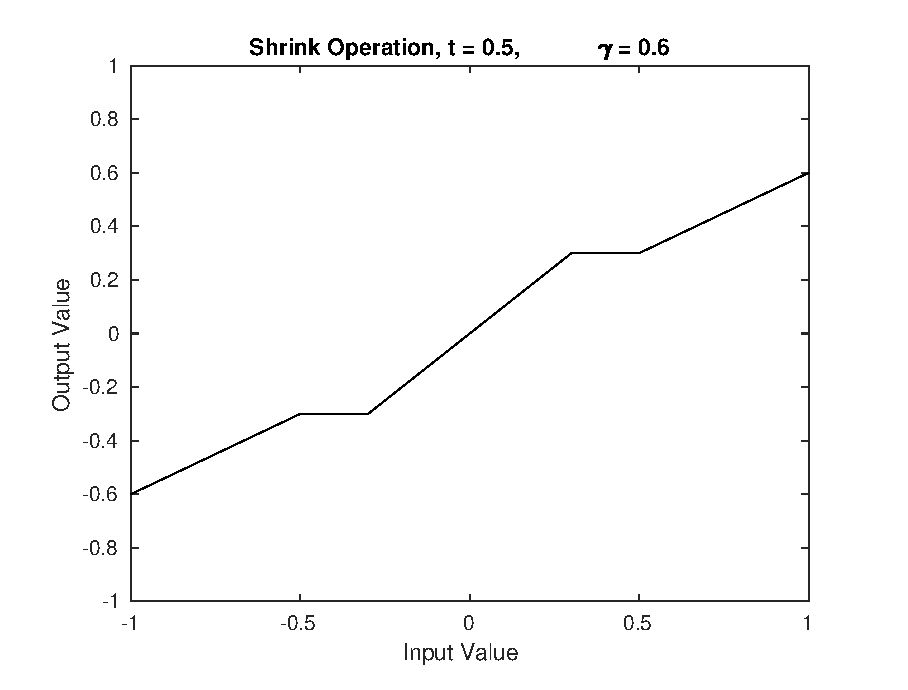
\includegraphics[width=0.45\textwidth]{shrink.eps}
  \caption{Shrink operation employed in the algorithm for $t = 0.5$, $\gamma = 0.6$.}
  \label{fig:shrink}
\end{figure}

The ``shrunken'' Gram matrix is then reduced to rank $p$ and decomposed into a squared-root matrix $S$ where $G = S^TS$.  $S$ is used to solve for the new projection matrix $P$ by finding the $P$ that minimizes $ || S - PD ||_F^2$.  All these steps together make up Elad's algorithm, described more formally here.  After Initialization of $P_0$ as a random matrix, for each iteration, $q$, do the following:
\begin{enumerate}
\item Normalize the columns of the effective dictionary $P_q D$ to obtain effective dictionary $\hat{D}$
\item Compute the Gram Matrix $G_q = \hat{D_q^T} \hat{D_q}$
\item Shrink the Gram matrix and obtain $\hat{G_q}$ by updating each entry according to $\hat{g_{ij}}$
\item Apply SVD and force rank of $\hat{G}$ to $p$
\item Find the squared-root $S_q \in \mathbb{R}^{p \times k}$ where $\hat{G_q} = S_q^TS_q$
\item Update $P_{q+1}$ by finding the $P$ that minimizes $|| S_q - PD ||_F^2$
\end{enumerate}

\section{IMPLEMENTATION}

Our implementation differed in a few important ways from that used in Elad's paper \cite{elad}.  First, the paper takes advantage of the fact that it is possible to determine $|| \alpha_j ||_0$ \emph{a priori} and generate sparse $\alpha_j$ with known $\ell_0$-norm.  Test signals $x_j$ may then be constructed accordingly.  Our implementation generated simple one to two tone signals $x_j = \sum_n sin(\omega_n t)$ that we assumed were sparse in the DCT.  This however led us to have $||\alpha_j||_0 \approx p$ while the paper could safely assume $ ||\alpha_j|| \ll p$, leading to improved reconstruction compared to ours.  Secondly, as our implementation did not use some of the BP optimizations exploiting known $||\alpha_j||_0$ values as the paper did, it ran an order of magnitude or more slower.  We thus reduced matrix sizes and signal averages in order to run the experiments in a reasonable time-frame, sacrificing favorable average mutual coherence of the effective dictionary leading to degraded reconstructions.  Finally, the paper operated in a second mode that accepted the parameter $t$ as a constant fraction of the entries in the Gram matrix to shrink.  This led to slightly improved convergence rates as compared to choosing a low threshold for $t$ and high choice of $\gamma$.

The algorith was straightforward to implement.  Steps 1--4 are easily implemented using MATLAB.  Step 5 is achieved through spectral decomposition of a semi-positive definite matrix with eigenvalues $\lambda_i$ and eigenvectors $v_i$ with $i = 1, \ldots p$: $$ \begin{aligned} \hat{G_q} &= \sum_{i=1}^p \lambda_i v_i^T v_i & \mbox{ with } y_i = {\lambda_i} v_i \\ &= \sum_{i=1}^p y_i^T y_i.  \end{aligned} $$  We then define $S_q$ to be the matrix whose columns are $y_i$, then it is clear that $S_q^T S_q = \hat{G}$.  Step 6 makes use of the Moore-Penrose pseudoinverse to solve $ P = S D^{-1} $.

\section{RESULTS}

We were able to successfully implement the algorithm as presented in the paper and observe similar results to those reported.  To show the behavior of our implementation, we constructed a random dictionary $D \in \mathbb{R}^{200 \times 400} $ with each entry drawn from an i.i.d. zero mean, unit variance Gaussian distribution with initial projection matrix $P \in \mathbb{R}^{30 \times 200}$ formed the same way.  After $400$ iterations and with appropriate choice of $t$ and $\gamma$, our algorithm produced a converging plot of $\mu_t\{PD\}$ as shown in Figure \ref{fig:mu_t}.  With increasing signal averages $x_j$, we anticipate that this curve would become increasingly smooth.

\begin{figure}[]
  \centering
  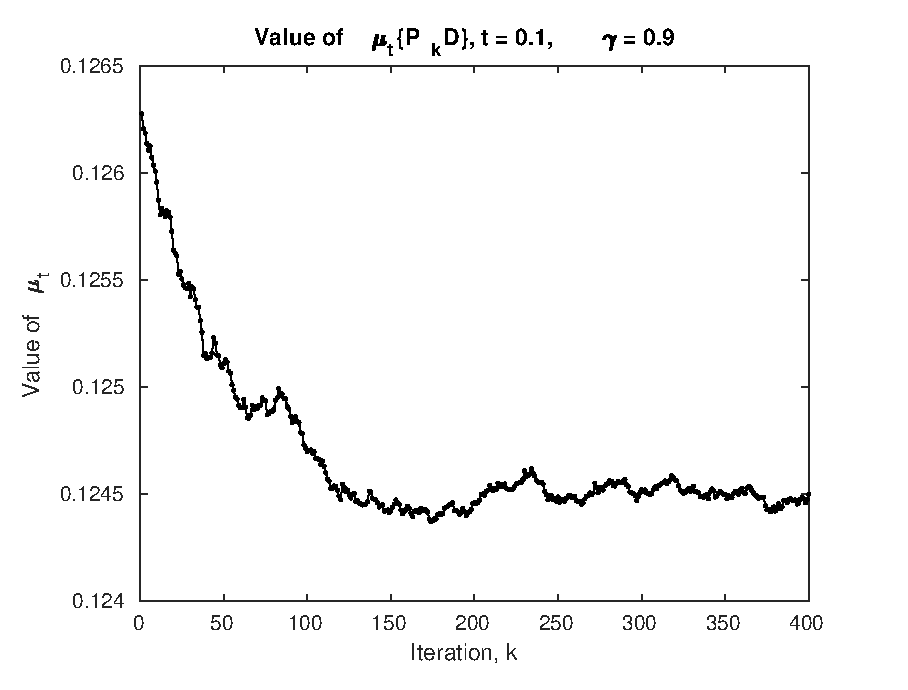
\includegraphics[width=0.45\textwidth]{mu_t_bw.eps}
  \caption{Value of $\mu_t\{P_kD\}$ as a function of the iteration for $t = 0.1$ and $\gamma = 0.9$.  As $k$ increases, $\mu_t$ converges to the value of $t$.}
  \label{fig:mu_t}
\end{figure}

Constructing a smaller $150 \times 250$ redundant DCT dictionary with $p$ varying from $21$--$25$, we found that optimizing $P$ with $200$ iterations and $15$ averaged test signals $x_j$ did indeed make an appreciable improvement over the reconstruction using only random choices of $P$.  Figure \ref{fig:err} shows the resultant CS reconstruction error as a function of $p$.  Although the difference between the error is small in our experiment, we observed that increasing the number of iterations, number of signal averages, and matrix dimensions increases the error gap and provides greater quality gains and more faithful reconstructions.  We did not run large experiments though, as these adjustments are computationally expensive, especially using our non-optimized numerical codes.

\begin{figure}[]
  \centering
  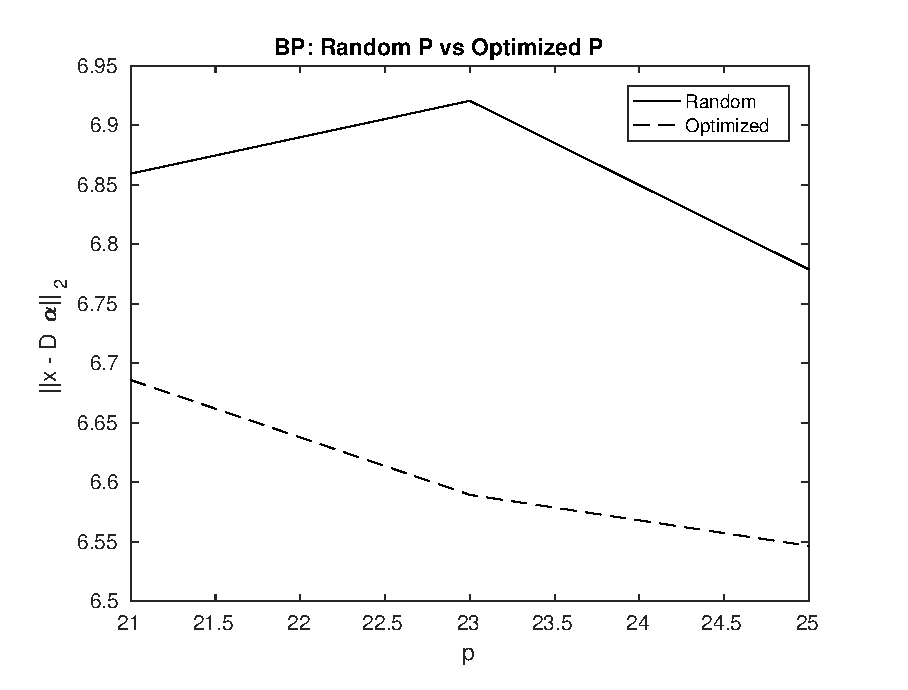
\includegraphics[width=0.45\textwidth]{rel_errors.eps}
  \caption{CS errors as a function of the number of measurements $p$ with randomly generated $P$ and optimized projections $P_{opt}$.}
  \label{fig:err}
\end{figure}

To visualize the change in the projection matrix $P$ after optimization, we recreated a histogram from the paper showing the absolute off-diagonal entries of the Gram matrix $G$ before and after the algorithm was run using a fixed $t$ value of $0.2$ and $\gamma$ of $0.4$.  Figure \ref{fig:hist} shows our results, which correspond well to results found in the paper.  We note a marked shift towards the origin of the histogram after optimization with a shortening of the tail (representing the ``shrinking'' of higher values in the Gram matrix).

\begin{figure}[]
  \centering
  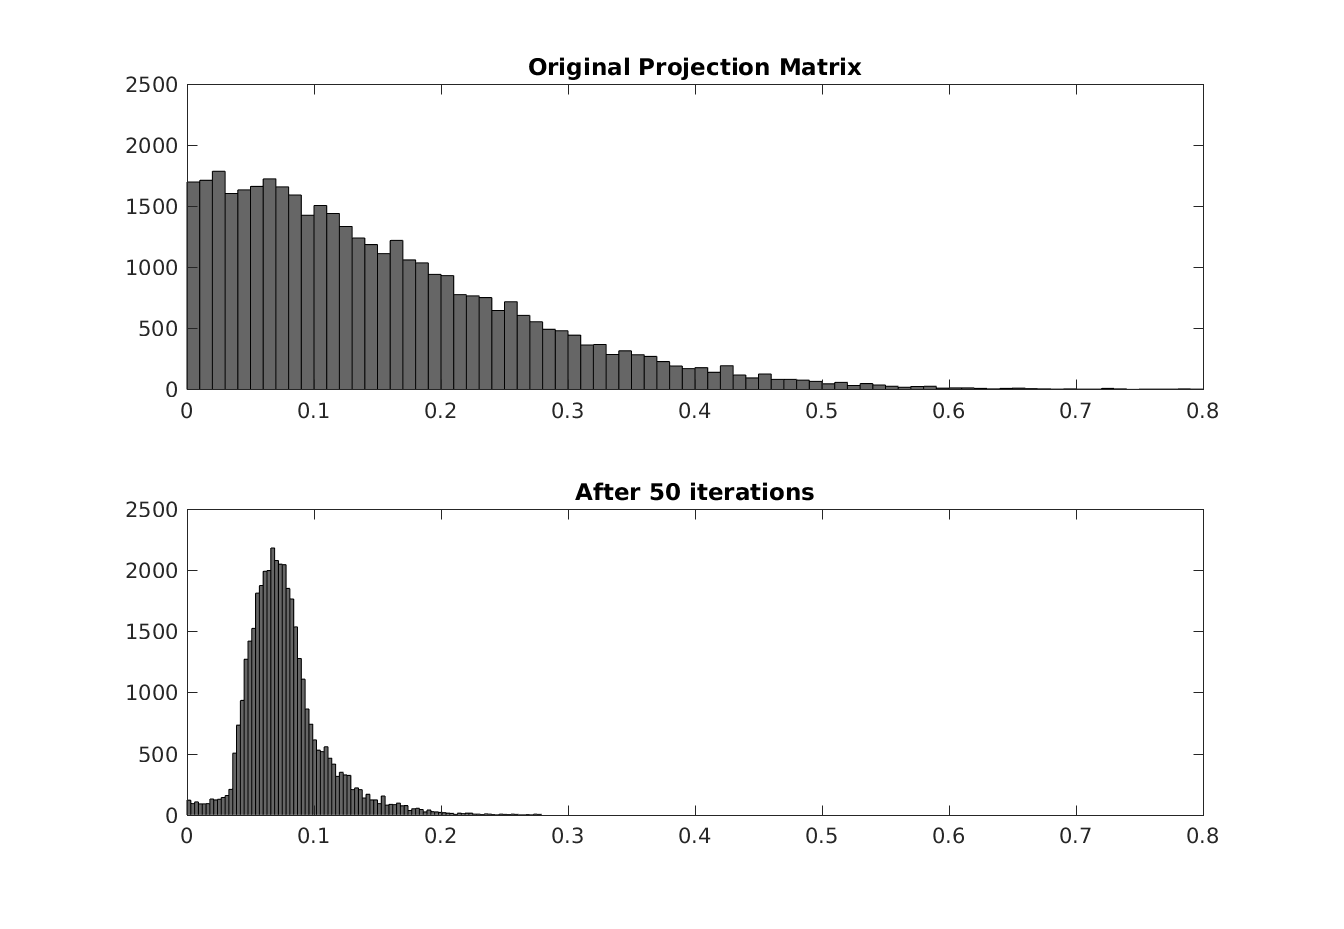
\includegraphics[width=0.45\textwidth]{hist_bw.eps}
  \caption{Histogram of the absolute off-diagonal entries of $G$ before the optimization and afterwards, using a fixed threshold $t = 0.2$.}
  \label{fig:hist}
\end{figure}

%%%%%%%%%%%%%%%%%%%%%%%%%%%%%%%%%%%%%%%%%%%%%%%%%%%%%%%%%%%%%%%%%%%%%%%%%%%%%%%%
\section{DISCUSSION}

There are several drawbacks to this algorithm.  The paper itself admits that it finds a suboptimal solution because the \emph{t}-averaged mutual coherence is quite different from the mutual coherence which is the real target \cite{lin}.  Second, Elad's algorithm provides no convergence guarantee for the \emph{t}-averaged mutual coherence and does not attempt to provide anything but empirical results.  Third, the selection of parameters $t$ and $\gamma$ are crucial for the performance of BP.  There is however no guideline for their settings and thus it is usually difficult to find their best choices.  But, Elad suggests that since the objective function can be evaluated after every iteration with minimal cost, this might be used to adjust the parameters dynamically after each iteration.

Despite its drawbacks, as a pioneering paper in mutual-coherence-based projection matrix optimization, Elad's work has laid the groundwork for research in this area of CS optimization \cite{tcs}.  Implementing this algorithm was an instructive exercise in the application of linear algebra to real research.

%%%%%%%%%%%%%%%%%%%%%%%%%%%%%%%%%%%%%%%%%%%%%%%%%%%%%%%%%%%%%%%%%%%%%%%%%%%%%%%%
\bibliographystyle{IEEEtran}
\bibliography{project}{}
%%%%%%%%%%%%%%%%%%%%%%%%%%%%%%%%%%%%%%%%%%%%%%%%%%%%%%%%%%%%%%%%%%%%%%%%%%%%%%%%

\end{document}
